\chapter{Graphical User Interface}

The user interface is divided in two windows: the ``Control Window'' and the ``Response Box''. The ``Control Window'' 
is used to set the experimental parameters, while the ``Response Box'' 
is the interface that the listeners use to give their responses.

\section{Quickstart}
When \texttt{pychoacoustics} is launched, the ``Control Window'' displays the default parameters for 
the ``Audiogram'' experiment. You can select another experiment using the ``Experiment'' 
drop-down menu, and edit any of the parameter fields you want to modify. Once you're 
satisfied with the parameters, you can store them by pressing the ``Store'' button. 
This stores one experimental block with the chosen parameters. At this point you 
can either start running the experiment by pressing the ``Start'' button on the 
``Response Box'', or you can add more experimental blocks by clicking on the ``New Block'' button.

To save the parameters to a file click on the ``Save Prm'' button. 
Parameter files that have been saved in this way can be later loaded 
into the program by using the ``Load Prm'' button.

To save the results of your experiment to a file, click on the ``Save Results'' button. 
If you have forgotten to specify a results file in this way, \texttt{pychoacoustics} 
will save the results in a file called \texttt{test.txt} in the working directory. 

\section{The Control Window}
The control window contains a set of widgets to manage the setup of the experiments,
running the experiments, processing results files and managing application preferences. 
Some of the widgets are general, and some of them are specific either to a given
paradigm (e.g.\ adaptive vs constant stimuli paradigm) or to a given experiment.

In the next section the function of these widgets will be explained, starting with the
widgets that are general to all experiments and paradigms.

\subsection{General Widgets (left panel)}
\label{sec:gui_left_panel}
\begin{itemize}
\item \textbf{Listener} This is simply a label that you can use to identify
the person who is running the experiment. This label will be written in the 
header of the results file.
\item \textbf{Experiment Label}. This is a label to identify the experiment 
you are running. This label will be written in the 
header of the results file.
\item \textbf{Session} This is a label to identify the experimental session,
it can be a number or a string. This label will be written in the 
header of the results file.
\item \textbf{Condition Label} This is a label to identify the experimental
condition of the current block of trials. It is optional, but it may be useful when
sorting the experimental results.
\item \textbf{End Command} Here you can write an operating system command 
(e.g.\ a bash command on Unix systems or a DOS command on Windows systems) to 
be performed at the end of the experimental session. 
This could be used to run a custom script to analyse the result files,
make a backup of the results files or other purposes. There are some variables
that can be accessed with a special string, such as the name of the results
file. These are listed in Section~\ref{sec:end_cmd} Table~\ref{tab:end_cmd}. Please, refer to that section 
for further info on how to use them. 

\item \textbf{Shuffling Scheme} By default when you click the ``Shuffle'' button, \texttt{pychoacoustics} randomly shuffles all blocks, here you can specify
different shuffling schemes (e.g.\ shuffle the first four blocks among themselves and the last four blocks among themselves).
Please refer to Section~\ref{sec:shuffling} for more details.

\item \textbf{Results File} Select a file for saving the results. Selecting an existing file will never
overwrite its content, it will simply append the new results to its content. If no file is selected,
the results will be saved in a file called \texttt{test.txt} in the current working directory. You can select
a file to save the results even after you have started a block of trials, the results get written to
the file only at the end of the block.

\item \textbf{Experimenter} Here you can select one of the experimenters listed in the
experimenter database. Please refer to Section~\ref{sec:experimenters_dialog} for further info on the experimenter
database and how it can be used. 
\item \textbf{Experiment} Selects the experiment for the current block.
\item \textbf{Paradigm} Selects the paradigm (e.g. adaptive, constant, etc\ldots) 
for the current block. The list of paradigms available depends on the experiment
that is selected. 
\item \textbf{Phones} Choose from one of the phone models stored in the phones database.
Please, refer to Section~\ref{sec:phones_dialog} for further info on how to enter phones and calibration values
in the database.
\item \textbf{Sample Rate (Hz)} Set the sampling rate of the sounds to be played. Any value
can be entered in the text fields. However, you should enter a value that is supported 
by your soundcard. A value that is not supported by your souncard may lead to issues,
although it's more likely that your soundcard will perform an automatic sample rate
conversion.
\item \textbf{Bits} Set the bit depth that \texttt{pychoacoustics} uses to store sounds 
to a wav file or play them. Currently values of 16 and 32 bits are supported. 
A value of 32 bits can be used for 24-bit soundcards. Notice that to achieve 24-bit output 
requires both a 24-bit souncard and a play command that can output 24-bit sounds. Therefore 
selecting a value of 32 bits here does not guarantee 24-bit playback even if you have a 24-bit souncard. 
Please, refere to Section~\ref{sec:sound_output} for further information on this issue.

\item \textbf{Repetitions} Set the number of times the sequence of blocks stored in memory should be repeated. If the ``Shuffle Mode'' (see below) is 
set to ``auto'', each time a new repetition starts the block positions will be shuffled. If the ``Shuffle Mode'' is set to ``Ask'', each time a new
repetition starts the user will be asked if s/he wants to shuffle the block positions. The ``Reset'' button resets the number of repetitions to zero.

\item \textbf{Pre-Trial Silence (ms)} Set a silent time interval before the start of each trial. 

\item \textbf{Warning Interval} Choose whether to present a warning light at the beginning of each trial. 

\item \textbf{Warning Interval Duration (ms)} Sets the duration of the warning interval light.
  This widget is shown only if the warning interval chooser is set to ``Yes''.

\item \textbf{Warning Interval ISI (ms)} Sets the duration of the silent interval between the end of warning interval and the start of the first observation interval.
  This widget is shown only if the warning interval chooser is set to ``Yes''.

\item \textbf{Pre-Trial Interval} Choose whether to present a pre-trial interval. This widget is shown only for experiments that have a pre-trial interval option.

\item \textbf{Pre-Trial Interval ISI (ms)} Sets the duration of the silent interval between the end of pre-trial interval and the start of the first observation interval.
  This widget is shown only if the current experiment has a pre-trial interval option and the pre-trial interval chooser is set to ``Yes''.

\item \textbf{Response Light} Set the type of response light at the end of each trial. "Feedback" will
flash a green (correct response) or red (incorrect response) light. "Neutral" will flash a white light.
"None" will not flash any light (there will nonetheless be a silent interval equal to the response light duration, see below).

\item \textbf{Response Light Duration (ms)} Set the duration of the response light.
 
\item \textbf{Shuffle Mode} If the ``Shuffle Mode'' is ``auto'', the  block presentation positions 
will be automatically shuffled at the beginning of a series of blocks. If the ``Shuffle Mode'' 
is ``Ask'', at the beginning of a series of blocks the user will be asked if the block presentation
positions should be shuffled or not. If the ``Shuffle Mode'' is ``No'', the block presentation positions
will not be automatically shuffled at the beginning of a series of blocks. 
See Section~\ref{sec:shuffling} for further information on shuffling the block presentation positions.

\item \textbf{Response Mode} When ``Real Listener'' is selected, \texttt{pychoacoustics} waits for responses
from a human listener. When ``Automatic'' is selected the program will give responses by itself with a certain
percentage correct, that can be specified in the ``Percent Correct (\%)'' text field. This mode is mostly
useful for debugging purposes, however it can also be used for experiments in which the
participants are passively listening to the stimuli (e.g. some neuroimaging experiments that record cerebral responses
rather than behavioural responses). In ``Simulated Listener'' mode \texttt{pychoacoustics} will give responses
on the bases of an auditory model. This model needs to be specified in the experiment file, the ``Simulated Listener'' mode
provides just a hook to redirect the control flow to your model.
Please, refer to Section~\label{sec:response_mode} for more information.


\end{itemize}

\subsection{General Widgets (right panel)}
\begin{itemize}
\item \textbf{Load Prm} Load in memory experimental parameters stored in a \texttt{.prm} file. See section~\ref{sec:parameters_files} for more info.
\item \textbf{Save Prm} Save experimental parameters stored in memory in a \texttt{.prm} file. See section~\ref{sec:parameters_files} for more info.
\item \textbf{Delete} Delete the current block from the blocks list.
\item \textbf{Undo Unsaved} Reset the parameters in the current block to the parameters that were last saved.
\item \textbf{Store} Store the parameters changes in memory.
\item \textbf{Store 'n' add} Store the parameter changes in memory and add a new parameters block.
\item \textbf{Store 'n' go} Store the parameter changes in memory and move to the next block storage point.
\item \textbf{New Block} Create a new parameters block (the parameters of the current block will be copied in the new one).
\item \textbf{Previous} Move to the previous block storage point.
\item \textbf{Next} Move to the next block storage point.
\item \textbf{Shuffle} Shuffle the block presentation positions.
\item \textbf{Reset} Reset the block presentation positions and move to the first block position.
\item \textbf{Jump to Block} Jump to a given block storage point.
\item \textbf{Previous Position} Move to the previous block presentation position.
\item \textbf{Next Position} Move to the next block presentation position.
\item \textbf{Jump to Position} Jump to the given block presentation position.
\item \textbf{Shift Blk. Down} Shift the current block to a lower storage point.
\item \textbf{Shift Blk. Up} Shift the current block to a higher storage point.
\end{itemize}

\subsection{Paradigm Widgets}
\subsubsection{Adaptive Paradigm Widgets}

\begin{itemize}
\item \textbf{Procedure} If ``Arithmetic'' the quantity defined by the step size will be added or subtracted to the parameter that is adaptively changing. 
  If ``Geometric'' the parameter that is adaptively changing will be multiplied or divided by the quantity defined by the step size.
\item \textbf{Initial Track Direction} This determines when the first turpoint will be called. If the initial track direction is ``Down'' the first turnpoint will be called
  the first time the adaptive track turns upward. If the initial track direction is ``Up'' the first turnpoint will be called
  the first time the adaptive track turns downward.
\item \textbf{Rule Down} Set the number of consecutive correct responses needed to subtract the current step size from the adaptive parameter (for arithmetic procedures) or divide
  the adaptive parameter by the current step size (for geometric procedures).
\item \textbf{Rule Up} Set the number of consecutive incorrect responses needed to add the current step size to the adaptive parameter (for arithmetic procedures) 
  or multiply the adaptive parameter by the current step size (for geometric procedures).
\item \textbf{Initial Turnpoints} Set the number of initial turnpoints. The initial turnpoints serve to bring quickly the adaptive track towards the listener's threshold.
  These turnpoints are not included in the threshold estimate. 
\item \textbf{Total Turnpoints} Set the number of total turnpoints. The number of total turnpoints is equal to the number of initial turnpoints that are not included in the threshold estimate
  plus the number of turnpoints that you want to use for the threshold estimate.
\item \textbf{Step Size 1} Set the step size for the initial turnpoints.
\item \textbf{Step Size 2} Set the step size to be used after the number of initial turnpoints has been reached.
\end{itemize}


\subsubsection{Weighted Up/Down Paradigm Widgets}

\begin{itemize}
\item \textbf{Procedure} If ``Arithmetic'' the quantity defined by the step size will be added or subtracted to the parameter that is adaptively changing. 
  If ``Geometric'' the parameter that is adaptively changing will be multiplied or divided by the quantity defined by the step size.
\item \textbf{Initial Track Direction} This determines when the first turpoint will be called. If the initial track direction is ``Down'' the first turnpoint will be called
  the first time the adaptive track turns upward. If the initial track direction is ``Up'' the first turnpoint will be called
  the first time the adaptive track turns downward.
\item \textbf{Percent Correct Tracked} Set the percentage correct point on the psychometric function to be tracked by the adaptive procedure. The ratio of the ``Up'' and ``Down'' steps
  is automatically adjusted by the software to satisfy this criterion.
\item \textbf{Initial Turnpoints} Set the number of initial turnpoints. The initial turnpoints serve to bring quickly the adaptive track towards the listener's threshold.
  These turnpoints are not included in the threshold estimate. 
\item \textbf{Total Turnpoints} Set the number of total turnpoints. The number of total turnpoints is equal to the number of initial turnpoints that are not included in the threshold estimate
  plus the number of turnpoints that you want to use for the threshold estimate.
\item \textbf{Step Size 1} Set the ``Down'' step size for the initial turnpoints. The ``Up'' step size is automatically calculated to satisfy the ``Percent Correct Tracked'' criterion.
\item \textbf{Step Size 2} Set the ``Down'' step size to be used after the number of initial turnpoints has been reached. The ``Up'' step size is automatically calculated to satisfy the ``Percent Correct Tracked'' criterion.
\end{itemize}
\subsubsection{Adaptive Interleaved Paradigm Widgets}

\begin{itemize}
\item \textbf{Procedure} If ``Arithmetic'' the quantity defined by the step size will be added or subtracted to the parameter that is adaptively changing. 
  If ``Geometric'' the parameter that is adaptively changing will be multiplied or divided by the quantity defined by the step size.
\item \textbf{No. Tracks} Set the number of adaptive tracks.
\item \textbf{Max. Consecutive Trials x Track} Set the maximum number of consecutive trials per track. 
\item \textbf{Turnpoints to Average} Since track selection is pseudo-random, it may happen that for a track the number of total turnpoints collected is greater
  than the number of total turnpoints requested for that track. If ``All final step size (even)'' is selected, the threshold will be estimated using all
  the turnpoints collected after the initial turnpoints, unless the number of these turnpoints is odd, in which case the first of these turnpoints will be discarded.
  If ``First N final step size'' is selected the threshold will be estimated using only the number of requested turnpoints collected after the initial turnpoints.
  If ``Last N final step size'' is selected the threshold will be estimated using only the last $N$ turnpoints, where $N$ equals the number of requested turnpoints.
\item \textbf{Initial Track X Direction} This determines when the first turpoint will be called for track number $X$. If the initial track direction is ``Down'' the first turnpoint will be called
  the first time the adaptive track turns upward. If the initial track direction is ``Up'' the first turnpoint will be called
  the first time the adaptive track turns downward.
\item \textbf{Rule Down Track X} Set the number of consecutive correct responses needed to subtract the current step size from the adaptive parameter (for arithmetic procedures) or divide
  the adaptive parameter by the current step size (for geometric procedures) for track number $X$.
\item \textbf{Rule Up Track X} Set the number of consecutive incorrect responses needed to add the current step size to the adaptive parameter (for arithmetic procedures) 
  or multiply the adaptive parameter by the current step size (for geometric procedures) for track number $X$.
\item \textbf{Initial Turnpoints Track X} Set the number of initial turnpoints for track number $X$. The initial turnpoints serve to bring quickly the adaptive track towards the listener's threshold.
  These turnpoints are not included in the threshold estimate. 
\item \textbf{Total Turnpoints Track X} Set the number of total turnpoints for track number $X$. The number of total turnpoints is equal to the number of initial turnpoints that are not included in the threshold estimate
  plus the number of turnpoints that you want to use for the threshold estimate.
\item \textbf{Step Size 1 Track X} Set the step size for the initial turnpoints for track number $X$.
\item \textbf{Step Size 2 Track X} Set the step size to be used after the number of initial turnpoints has been reached for track number $X$.
\end{itemize}

\subsubsection{Weighted Up/Down Interleaved Paradigm Widgets}

\begin{itemize}
\item \textbf{Procedure} If ``Arithmetic'' the quantity defined by the step size will be added or subtracted to the parameter that is adaptively changing. 
  If ``Geometric'' the parameter that is adaptively changing will be multiplied or divided by the quantity defined by the step size.
\item \textbf{No. Tracks} Set the number of adaptive tracks.
\item \textbf{Max. Consecutive Trials x Track} Set the maximum number of consecutive trials per track. 
\item \textbf{Turnpoints to Average} Since track selection is pseudo-random, it may happen that for a track the number of total turnpoints collected is greater
  than the number of total turnpoints requested for that track. If ``All final step size (even)'' is selected, the threshold will be estimated using all
  the turnpoints collected after the initial turnpoints, unless the number of these turnpoints is odd, in which case the first of these turnpoints will be discarded.
  If ``First N final step size'' is selected the threshold will be estimated using only the number of requested turnpoints collected after the initial turnpoints.
  If ``Last N final step size'' is selected the threshold will be estimated using only the last $N$ turnpoints, where $N$ equals the number of requested turnpoints.
\item \textbf{Initial Track X Direction} This determines when the first turpoint will be called for track number $X$. If the initial track direction is ``Down'' the first turnpoint will be called
  the first time the adaptive track turns upward. If the initial track direction is ``Up'' the first turnpoint will be called
  the first time the adaptive track turns downward.
\item \textbf{Percent Correct Tracked} Set the percentage correct point on the psychometric function to be tracked by the adaptive procedure for track number $X$. The ratio of the ``Up'' and ``Down'' steps
  is automatically adjusted by the software to satisfy this criterion.
\item \textbf{Initial Turnpoints Track X} Set the number of initial turnpoints for track number $X$. The initial turnpoints serve to bring quickly the adaptive track towards the listener's threshold.
  These turnpoints are not included in the threshold estimate. 
\item \textbf{Total Turnpoints Track X} Set the number of total turnpoints for track number $X$. The number of total turnpoints is equal to the number of initial turnpoints that are not included in the threshold estimate
  plus the number of turnpoints that you want to use for the threshold estimate.
\item \textbf{Step Size 1 Track X} Set the ``Down'' step size for the initial turnpoints for track number $X$. The ``Up'' step size is automatically calculated to satisfy the ``Percent Correct Tracked'' criterion.
\item \textbf{Step Size 2 Track X} Set the ``Down'' step size to be used after the number of initial turnpoints has been reached for track number $X$. The ``Up'' step size is automatically calculated to satisfy the ``Percent Correct Tracked'' criterion.
\end{itemize}


\subsubsection{Constant m-Intervals n-Alternatives Paradigm Widgets}

\begin{itemize}
\item \textbf{No. Trials} Set the number of trials to be presented in the current block.
\item \textbf{No. Practice Trials} Set the number of practice trials to be presented in the current block. Practice trials are presented at the
  beginning of the block; the responses to these trials are not included in the statistics.
\end{itemize}

\subsubsection{Multiple Constants m-Intervals n-Alternatives Paradigm Widgets}

\begin{itemize}
\item \textbf{No. Trials} Set the number of trials to be presented in the current block for each condition.
\item \textbf{No. Practice Trials} Set the number of practice trials to be presented in the current block for each condition. The responses to these trials are not included in the statistics.
\item \textbf{No. Differences} Set the number of conditions to be used in the current block.
\end{itemize}

\subsubsection{Constant 1-Interval 2-Alternatives Paradigm Widgets}

\begin{itemize}
\item \textbf{No. Trials} Set the number of trials to be presented in the current block.
\item \textbf{No. Practice Trials} Set the number of practice trials to be presented in the current block. Practice trials are presented at the
  beginning of the block; the responses to these trials are not included in the statistics.
\end{itemize}

\subsubsection{Multiple Constants 1-Interval 2-Alternatives Paradigm Widgets}

\begin{itemize}
\item \textbf{No. Trials} Set the number of trials to be presented in the current block for each condition.
\item \textbf{No. Practice Trials} Set the number of practice trials to be presented in the current block for each condition. The responses to these trials are not included in the statistics.
\item \textbf{No. Differences} Set the number of conditions to be used in the current block.
\end{itemize}

\subsubsection{1-Pair Same/Different Paradigm Widgets}

\begin{itemize}
\item \textbf{No. Trials} Set the number of trials to be presented in the current block.
\item \textbf{No. Practice Trials} Set the number of practice trials to be presented in the current block. Practice trials are presented at the
  beginning of the block; the responses to these trials are not included in the statistics.
\end{itemize}

\subsection{The Menu Bar}
A screenshot of the menu bar is shown in Figure~\ref{fig:menuBar}. This bar is located in the upper left corner of the ``Control Window''. Each menu will be described below.
\begin{figure}[!h]
   \caption{The menu bar.}
   \centering
   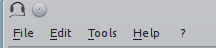
\includegraphics{Figures/menuBar.png}
   \label{fig:menuBar}
 \end{figure}

\subsubsection{The File Menu}
\begin{itemize}
\item \textbf{Process Results} Process block summary results files to obtain 
session summary results files. For more info see Section~\ref{sec:proc_res_dia}.
\item \textbf{Process Results Table} Process block summary results table files to obtain 
session summary table results files. For more info see Section~\ref{sec:proc_res_dia}.
\item \textbf{Open Results File} Open the file where \texttt{pychoacoustics} is currently saving data with the default text editor.
\item \textbf{Exit.} Close \texttt{pychoacoustics}.

\end{itemize}

\subsubsection{The Edit Menu}
\begin{itemize}
\item \textbf{Edit Preferences} Edit application preferences. See Section~\ref{sec:pref_dialog} for further info.
\item \textbf{Edit Phones} Edit the phones database, and set the calibration levels for your phones. See Section~\ref{sec:phones_dialog} for further info.
\item \textbf{Edit Experimenters} Edit the experimenters database. See Section~\ref{sec:experimenters_dialog} for further info.
\end{itemize}

\subsubsection{The Tools Menu}
\begin{itemize}
\item \textbf{Swap Blocks} Swap the storage position of two parameter blocks.
\end{itemize}

\subsubsection{The Help Menu}
\begin{itemize}
\item \textbf{Fortunes} Show psychoacoustics fortunes. I'm always collecting new ones, so if you happen to know any interesting ones, please, e-mail them to me so that I can add them to the collection.
\item \textbf{About pychoacoustics} Show information about the licence, the version of the software and the version of the libraries it depends on.
\end{itemize}

\subsubsection{The ``what's this?'' Button.}
If you click on this button, and then click on a widget,
you can get some information about the widget (this is not implemented
for all widgets).

\section{Process Results Dialog}
\label{sec:proc_res_dia}
Figure~\ref{fig:proc_res_dia} show a screenshot of the process results dialog. The dialog is the same for all
procedures, except that for procedures in which \emph{d'} is computed, there is an additional checkbox asking whether to
apply a correction to hit/false alarm rates of zero or one. For information on the format of the result files,
please see Section~\ref{sec:results_files}. 
\begin{figure}[!h]
   \caption{The process results dialog.}
   \centering
   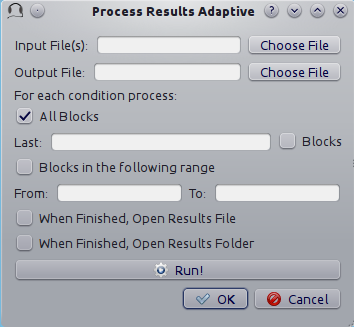
\includegraphics{Figures/proc_res_dia.png}
   \label{fig:proc_res_dia}
 \end{figure}
\begin{itemize}
\item \textbf{Input File(s)} Give the filepath of one or more files to be processed. The ``Choose File'' button can be used to select the file(s). Multiple filepaths
  should be separated by a semicolon ``\texttt{;}''.
\item \textbf{Output File} Give the filename of the output file.
\item \textbf{For each condition process:}
  \begin{itemize}
  \item \textbf{All Blocks} If checked, all blocks in the result file(s) will be processd.
  \item \textbf{Last X Blocks} If checked, only the last $X$ blocks will be processed.
  \item \textbf{Blocks in the following range} If checked, only blocks in the specified range will be processed (indexing starts from 1).
  \end{itemize}
\item \textbf{d-prime correction} If checked, convert hit rates of $0$ and $1$ to $1/2N$ and $1-1/(2N)$ respectively, where $N$ is the number of trials, to avoid infinite values of \emph{d'} \cite<see>[p.\ 8]{Macmillan2005}.
  This checkbox is available only for some paradigms.
\item \textbf{When finished, open results file} If checked, the output file will be opened in the default text editor when processing has finished.
\item \textbf{When finished, open results folder} If checked, the folder containing the output file will be opened when processing has finished.
\item \textbf{Run!} Click this button to process the result files.
 
\end{itemize}


\section{Edit Preferences Dialog}
\label{sec:pref_dialog}
The preferences dialog is divided into several tabs. These are described in turn below.

\subsection{General}
\label{sec:pref_dialog_gen}
\begin{itemize}
\item \textbf{Language (requires restart)} Choose the application language. At the moment and for the foreseeable future
  only English is supported.
\item \textbf{Country (requires restart)} Set the country locale to be used for the application. Some things (e.g.\ the way dates are written in result files depend on this setting.
\item \textbf{Response Box Language (requires restart)} Choose the language to be used for the ``Response Box''. This set the language to be used for the button labels and other
  GUI elements that the experimental listener is presented with. 
\item \textbf{Response Box Country (requires restart)} Set the country locale for the response box.
\item \textbf{csv separator} Choose the separator field to be used  when writing the csv tabular result files.
\item \textbf{Warn if listener name missing} If checked, pop up a warning message if the listener name is missing at the beginning of a session.
\item \textbf{Warning if session label missing} If checked, pop up a warning message if the session label is missing at the beginning of a session.
\item \textbf{Process results when finished} If checked, process automatically the block summary file to generate the session summary file at the end of the experiment.
\item \textbf{d-prime correction} If checked, when automatically processing result files, convert hit rates of $0$ and $1$ to $1/2N$ and $1-1/(2N)$ respectively, where $N$ is the number of trials, to avoid infinite values of \emph{d'} \cite<see>[p.\ 8]{Macmillan2005}.
\item \textbf{Max Recursion Depth (requires restart)} Set the maximum recursion depth of the Python interpreter stack. This setting should be changed only if you intend
  to run \texttt{pychoacoustics} in automatic or simulated listener response mode. Beware, setting a max recursion depth value smaller than the default value may cause
  \texttt{pychoacoustics} to crash or not even start. In case \texttt{pychoacoustics} does not start because of this, delete your preferences settings file to restore
  the default max recursion depth value.
 
\end{itemize}

\subsection{Sound}
\label{sec:pref_dialog_sound}
\begin{itemize}
\item \textbf{Play Command} Set an internal or external command to play sounds.
\item \textbf{Device} Set the soundcard to be used to play sounds. This chooser is available
  only for certain internal play commands (currently alsaaudio and pyaudio).
\item \textbf{Buffer Size (samples)} Set the buffer size in number of samples to be used to output sounds. This chooser is available only for certain internal play commands (currently alsaaudio and pyaudio).
\item \textbf{Default Sampling Rate} Set the default sampling rate.
\item \textbf{Default Bits} Set the default bit depth.
\item \textbf{Wav manager (requires restart)} Choose the wav manager.
\item \textbf{Write wav file} Write wav files with the sounds played on each trial in the current \texttt{pychoacoustics} working directory.
\item \textbf{Write sound sequence segment wavs} For sound sequences, write a wav file for each segment of the sequence in the current \texttt{pychoacoustics} working directory.
\item \textbf{Append silence to each sound (ms)} Append a silence of the given duration at the end of each sound. This is useful on some versions of the Windows operating system that may cut the sound buffer before it has ended resulting in audible clicks.
\end{itemize}

\subsection{Notifications}
\label{sec:pref_dialog_notify}
\begin{itemize}
\item \textbf{Play End Message} If checked, play a wav file at the end of the experiment.
  This could be short message to let the listeners know they have finished and thank them
  for their participation in the experiment. One or more wav files need to be set through
  the ``Choose wav'' button for this work.
\item \textbf{Choose wav} Choose the wav file to be played as the end message. Clicking on this button 
  brings up another dialog where you can select the wav files to be played and their output RMS.
  Only one of the wav files listed here and with the ``Use'' flag set to \ding{51} will be randomly chosen
  and played.
\item \textbf{blocks before end of experiment} Set how many blocks before the end of the experiment
  the two actions listed below (send notification e-mail and execute custom command) should be performed.
\item \textbf{Send notification e-mail} If checked, send a notification e-mail to the experimenter
  to notify her that the experiment is about to finish.
\item \textbf{Execute custom command} If checked, execute an operating system command before the end
  of the experiment. This command could be used to automatically send an sms for example.
\item \textbf{Send data via e-mail} At the end of the experiment, send the results file to the experimenter .
\item \textbf{Execute custom command} At the end of the experiment, execute an operating system command.
\item \textbf{Outgoing Server (SMTP)} Set the name of the SMTP server to be used by \texttt{pychoacoustics} to send e-mails.
\item \textbf{Port} Set the port number for the SMTP server.
\item \textbf{Security} Set the security protocol for network exchanges with the SMTP server.
\item \textbf{Server requires identification} Check this if the SMTP server requires identification.
\item \textbf{Username} Set the username for the SMTP server.
\item \textbf{Password} Set the password for the SMTP server.
\item \textbf{Send test e-mail} Send a test e-mail to check that the server settings are OK.
\end{itemize}

\subsection{EEG}
\label{sec:pref_dialog_eeg}
\begin{itemize}
\item \textbf{ON Trigger} The ON trigger value (decimal).
\item \textbf{OFF Trigger} The OFF trigger value (decimal).
\item \textbf{Trigger Duration (ms)} The duration of the trigger in milliseconds.
\end{itemize}


\section{Edit Phones Dialog}
\label{sec:phones_dialog}
A screenshot of the ``Edit Phones'' dialog is shown in Figure~\ref{fig:phones_dialog}.
\begin{figure}[!hbt]
   \caption{The edit phones dialog.}
   \centering
   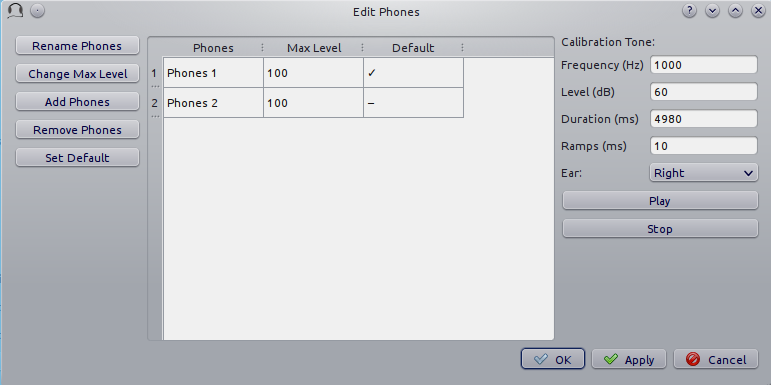
\includegraphics[scale=.65]{Figures/phones_database.png}
   \label{fig:phones_dialog}
 \end{figure}
Most of the fields should be pretty much self-explanatory. Using this dialog you can add headphones/earphones
models to the phones database. The phone with the ``Default'' flag set to \ding{52} will be selected by default when \texttt{pychoacoustics} is started. In the ``Max Level'' field you should enter the level in dB SPL that is output by the phone for a full amplitude sinusoid. This value will be used by \texttt{pychoacoustics} to output sounds at specific levels in dB SPL. On the rightmost panel of the dialog you have facilities to play a sinusoid with a specified level. You can use these facilities to check with a SPL meter (or a voltmeter depending on how you're doing it) that the actual output level corresponds to the desired output level. Using these facilities you can also play a full amplitude sinusoid: you need to set the level of the sinuoid to the ``Max Level'' of the phone (whatever it is). Be careful because it can be very loud!

\section{Edit Experimenters Dialog}
\label{sec:experimenters_dialog}
A screenshot of the ``Edit Experimenters'' dialog is shown in Figure~\ref{fig:experimenters_dialog}.
\begin{figure}[!h]
   \caption{The edit experimenters dialog.}
   \centering
   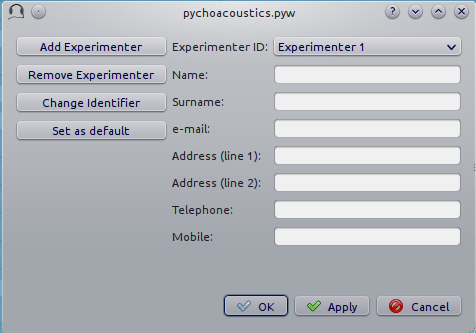
\includegraphics{Figures/experimenter_database.png}
   \label{fig:experimenters_dialog}
 \end{figure}
Most of the fields should be pretty much self-explanatory. Here you can add
the details of the experimenters that work in your lab in the experimenter
database. The main functions of this database at the moment are a) writing
the experimenter name in the results file; b) using the experimenter e-mail 
for sending notifications and/or results files (see Section~\ref{sec:pref_dialog_notify}).



\section{The Response Box}

The ``response box'' consists of a large button (the ``status button'') that is used to start a block of trials, a feedback light to display trial by trial feedback, interval lights to mark observation intervals, and response buttons. The responses can be given either by means of mouse clicks, or using the numeric keypad (key ``1'' for the first button, key ``2'' for the second button etc\ldots). Responses given before all observation intervals have been presented are not accepted. 

The status button can be activated  by pressing the \texttt{Ctrl+R} shortcut.  At the start of each block the label of the ``Status Button'' is set to ``Start''. Once the listener starts a block of trials the label of the status button changes to ``Running''. When a whole series of blocks is finished the label of the status button changes to ``Finish''. If no blocks are stored in memory the label of the status button is set to ``Wait''.

On the top left corner of the response box there is a semi-hidden menu signalled by a little hyphen (``-''). If you click on it you have access to two functions. The ``Show/Hide Control Window'' function can be used to hide the control window while the experiment is running. This is useful because it prevents the listener from accidentally changing your experimental parameters or accidentally closing \texttt{pychoacoustics} (the response box itself has no ``close'' button, so it is not possible to close that). The ``Show/Hide progress Bar'' function can be used to display a progress bar at the bottom of the response box. The progress bar estimates what percentage of the experiment has been completed. This estimate depends on the procedure used (for constant procedures it is based on the number of trials done, while for adaptive procedures it is based on the number of turnpoints reached) and on the specific parameters of a given experiment (trial duration, number of trials, or number or turnpoints, all of which can differ between blocks), so in some cases the estimate can be off the mark. The ``Show/Hide block progress Bar'' can be used to show the position of the current block and the total number of blocks. 





%%% Local Variables: 
%%% mode: latex
%%% TeX-master: "pychoacoustics_manual"
%%% End: 
